\documentclass[a4paper, 12pt, english]{article}

% \usepackage[portuges]{babel}
\usepackage[utf8]{inputenc}
\usepackage{amsmath,amssymb}
\usepackage{graphicx}
\usepackage{subfig}
\usepackage[colorinlistoftodos]{todonotes}

\usepackage{indentfirst}
\usepackage{verbatim}
\usepackage{textcomp}
\usepackage{gensymb}
\usepackage{float}
\usepackage{pgfplots}
\pgfplotsset{compat=1.17}

\usepackage{relsize}

\usepackage{lipsum}% http://ctan.org/pkg/lipsum
\usepackage{xcolor}% http://ctan.org/pkg/xcolor
\usepackage{xparse}% http://ctan.org/pkg/xparse
\NewDocumentCommand{\myrule}{O{1pt} O{2pt} O{black}}{%
	\par\nobreak % don't break a page here
	\kern\the\prevdepth % don't take into account the depth of the preceding line
	\kern#2 % space before the rule
	{\color{#3}\hrule height #1 width\hsize} % the rule
	\kern#2 % space after the rule
	\nointerlineskip % no additional space after the rule
}
\usepackage[section]{placeins}

\usepackage{booktabs}
\usepackage{colortbl}%
\newcommand{\myrowcolour}{\rowcolor[gray]{0.925}}

\usepackage[obeyspaces]{url}
\usepackage{etoolbox}
\usepackage[colorlinks,citecolor=black,urlcolor=blue,bookmarks=false,hypertexnames=true]{hyperref}

\usepackage{geometry}
\geometry{
	paper=a4paper, % Change to letterpaper for US letter
	inner=3cm, % Inner margin
	outer=3cm, % Outer margin
	bindingoffset=.5cm, % Binding offset
	top=2cm, % Top margin
	bottom=2cm, % Bottom margin
	%showframe, % Uncomment to show how the type block is set on the page
}
\usepackage{fancyhdr}

% Define header and footer
\pagestyle{fancy}
\fancyhf{}
\lhead{ENER 104L}
\rhead{iSciM, Habib University} % Right-aligned page number in the header
\rfoot{\thepage} % Right footer text
%*******************************************************************************%
%************************************START**************************************%
%*******************************************************************************%
\begin{document}

%************************************TITLE PAGE**************************************%
\begin{titlepage}
	\begin{center}
		\textbf{\LARGE Habib University}\\[0.5cm]
		\textbf{\large iSciM}\\[0.2cm]
		\textbf {\large Fall 2023}\\[0.2cm]
		\vspace{20pt}
		
\includegraphics[width=5cm]{../habiblogo.jpg}\\[1cm]
		\par
		\vspace{20pt}
		\textbf{\Large ENER 104L RENEWABLE ENERGY}\\
		\vspace{15pt}
		\myrule[1pt][7pt]
		\textbf{\LARGE  LABORATORY REPORT 5}\\
		\vspace{15pt}
		\textbf{\large Electrical Energy from Solar Energy}\\
		\myrule[1pt][7pt]
		\vspace{25pt}
		\begin{tabular}{@{}p{5cm}p{3cm}@{}}
			\textbf{\large Student Name} & \textbf{\large Student ID} \\
			Ali Asghar Yousuf            & ay06993                    \\ % No1 
			Syed Ibrahim Ali Haider      & sh06565                    \\ % No2
		\end{tabular}

		\vspace{10pt}
		\begin{tabular}{@{}p{5cm}p{3cm}@{}}
			\textbf{\large Group Name} & \textbf{\large Group No.} \\
			Insane Fr                  & 1                         \\
		\end{tabular}

		\vspace{45pt}
		\textbf {\large Lab Instructors:}\\[0.2cm]
		\Large {Paishwa Naqvi}\\[0.1cm]
		\Large {Amber Talat}\\[0.1cm]
		\Large {Mah Noor Jamil}\\[0.1cm]
	\end{center}

	\par
	\vfill
	\begin{center}
		\textbf{\today}\\
	\end{center}

\end{titlepage}

%************************************TABLE OF CONTENTS**************************************%

%  %Sumário
%  \newpage
%  \tableofcontents
%  \thispagestyle{empty}
%  %End Sumário

%********************************%
%***********SECTION 1************%
%********************************%
\newpage
\section{Objectives}
\begin{itemize}
	\item To understand the basic operation of a solar cell.
	\item To understand the influence of illumination level on the output voltage and
	      current of a solar cell.
	\item To understand the influence of the area of illumination on the output voltage
	      and current of a solar cell.
	\item To understand the influence of illumination intensity and distance from the
	      light source on the output voltage and current of a solar cell.
\end{itemize}

\section{Abstract}
The objective of this lab was to understand the working of a solar cell and how
the output voltage and current of a solar cell is affected by the illumination
level, area of illumination, illumination angle and distance from the light
source. The solar cell was connected to a multimeter and the output voltage and
current were measured for different illumination levels, areas of illumination,
illumination angles and distances from the light source.

\section{Result and Analysis}
\subsection{Part A}
In the first part of the experiment, the solar cell was connected to a
multimeter and the output voltage and current were measured for different
distances from the light source, as the distance from the light source
increased, the illumination intensity reaching the solar cell decreased. The
results are shown in Table \ref{tab:Table 1}.

\begin{table}[H]
	\caption{\label{tab:Table 1} Voltage \& Current Table}
	\centering
	\begin{tabular}{c c c}
		\toprule
		\textbf{Position}
		           & \textbf{Voltage (V)}
		           & \textbf{Current (mA)}         \\
		\cmidrule[0.4pt](r{0.125em}){1-1}%
		\cmidrule[0.4pt](lr{0.125em}){2-2}%
		\cmidrule[0.4pt](lr{0.125em}){3-3}%
		% \midrule
		\textbf{1} & 0.65                  & 260.0 \\
		\textbf{2} & 0.62                  & 151.4 \\
		\textbf{3} & 0.60                  & 100.4 \\
		\bottomrule
	\end{tabular}
\end{table}

We observed that as the distance from the light source increased, the output
voltage saw a slight decrease which can be attributed to experimental error,
however, the output current saw a significant decrease as the distance from the
light source increased. This is because the illumination intensity reaching the
solar cell decreased as the distance from the light source increased, which
resulted in a decrease in the output current.

\begin{figure}[H]
	\centering
	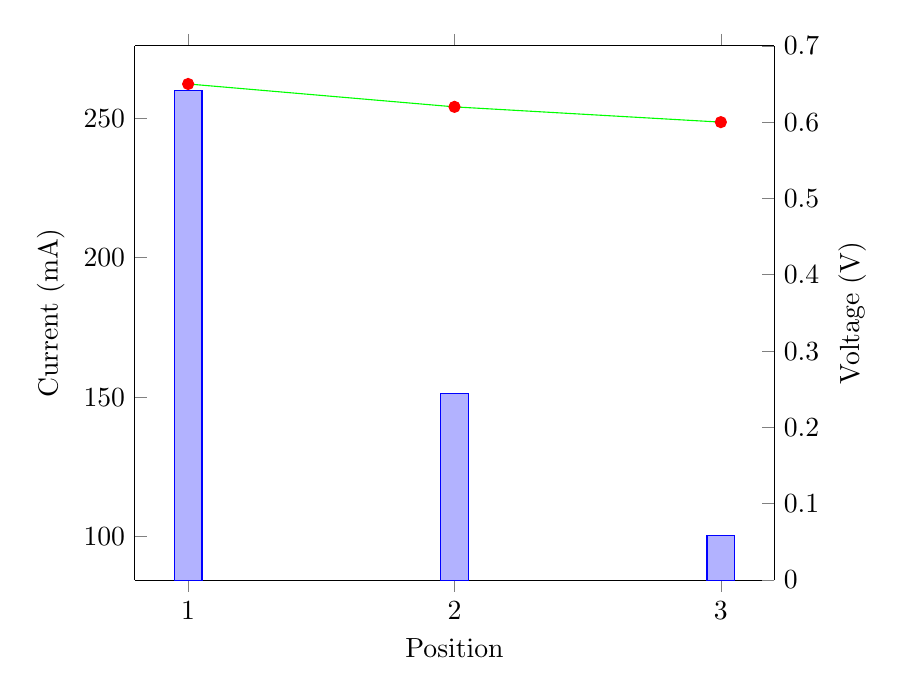
\begin{tikzpicture}
		\begin{axis}[
				width=0.8\textwidth,
				ybar,
				xlabel=Position,
				xtick=data,
				xticklabels= {1, 2, 3},
				axis y line*=left,
				ylabel=Current (mA),
			]

			\addplot table[x expr=\coordindex, y=Current] {
					Position Current
					1        260.0
					2        151.4
					3        100.4
				};
		\end{axis}

		\begin{axis}[
				width=0.8\textwidth,
				% ybar,
				ylabel=Voltage (V), axis y line*=right, ymin=0.0, ymax=0.7, axis x line=none,
				% enlarge x limits=0.15,
			]

			\addplot[mark=*, mark options={color=red}, draw=green] table[x expr=\coordindex, y=Voltage] {
					Position Voltage
					1        0.65
					2        0.62
					3        0.60
				};
		\end{axis}
	\end{tikzpicture}
	\caption{Current and Voltage Bar Chart}
\end{figure}

\subsection{Part B}
In the second part of the experiment, the solar cell was connected to a
multimeter and the output voltage and current were measured for different areas
of illumination. The solar cell was covered with a cardboard sheet and the
cardboard sheet was gradually removed to uncover different areas of the solar
cell. The results are shown in Table \ref{tab:Table 2}.

\begin{table}[H]
	\caption{\label{tab:Table 2} Voltage \& Current Table}
	\centering
	\begin{tabular}{c c c}
		\toprule
		\textbf{Area Uncovered}
		               & \textbf{Voltage (V)}
		               & \textbf{Current (mA)}         \\
		\cmidrule[0.4pt](r{0.125em}){1-1}%
		\cmidrule[0.4pt](lr{0.125em}){2-2}%
		\cmidrule[0.4pt](lr{0.125em}){3-3}%
		% \midrule
		1              & 0.65                  & 260.0 \\
		$\dfrac{3}{4}$ & 0.61                  & 125.0 \\
		$\dfrac{1}{2}$ & 0.59                  & 70.5  \\
		$\dfrac{1}{4}$ & 0.57                  & 40.2  \\
		\bottomrule
	\end{tabular}
\end{table}

We observed that as the uncovered area of the solar cell decreased, the output
voltage saw a slight decrease which can be attributed to experimental error,
however, the output current saw a significant decrease as the uncovered area of
the solar cell decreased. This is because the illumination intensity reaching
the solar cell decreased as the uncovered area of the solar cell decreased,
which resulted in a decrease in the output current.

\begin{figure}[H]
	\centering
	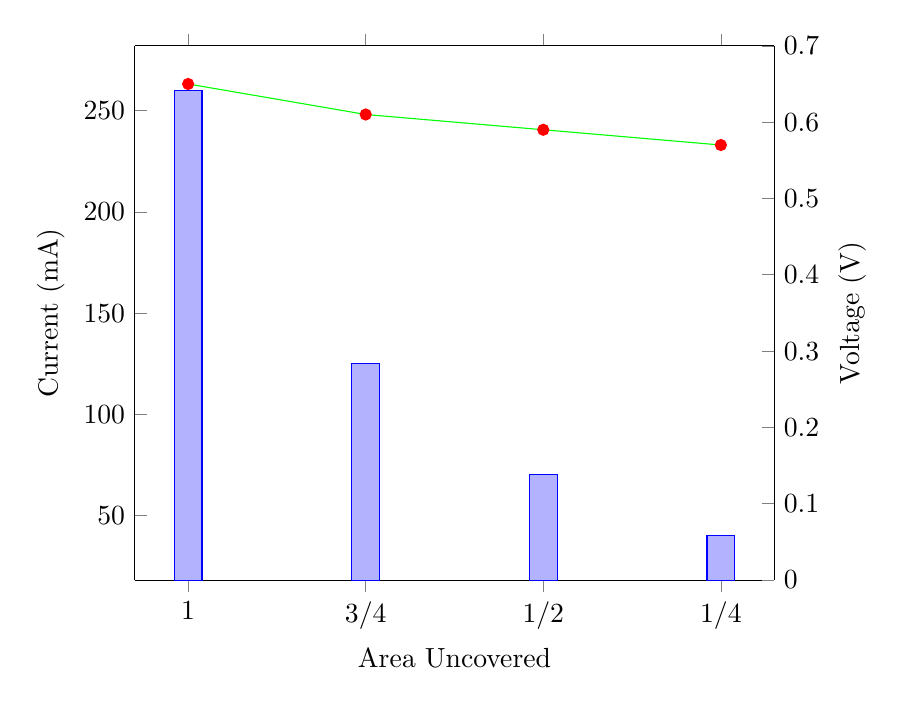
\begin{tikzpicture}
		\begin{axis}[
				width=0.8\textwidth,
				ybar,
				xlabel=Area Uncovered,
				xtick=data,
				xticklabels= {1, 3/4, 1/2, 1/4},
				axis y line*=left,
				ylabel=Current (mA),
			]

			\addplot table[x expr=\coordindex, y=Current] {
					Area Current
					1    260.0
					2    125.0
					3    70.5
					4    40.2
				};
		\end{axis}

		\begin{axis}[
				width=0.8\textwidth,
				% ybar,
				ylabel=Voltage (V), axis y line*=right, ymin=0.0, ymax=0.7, axis x line=none,
				% enlarge x limits=0.15,
			]

			\addplot[mark=*, mark options={color=red}, draw=green] table[x expr=\coordindex, y=Voltage] {
					Area Voltage
					1    0.65
					2    0.61
					3    0.59
					4    0.57
				};
		\end{axis}
	\end{tikzpicture}
	\caption{Current and Voltage Bar Chart}
\end{figure}

\section{Conclusion}
With the help of this experiment, we were able to understand the working of a
solar cell and our readings were consistent with our expectations. As the
distance from the light source increased, the illumination intensity reaching
the solar cell decreased, which resulted in a decrease in the output current.
Similarly, as the uncovered area of the solar cell decreased, the illumination
intensity reaching the solar cell decreased, which resulted in a decrease in
the output current. While the output voltage remained relatively constant in
both cases.

\end{document}